\chapter{Программное обеспечение}
\label{ch:chap2}
В этой главе описываются принципы работы с ROS2 (Robotic Operating System) - программное обеспечение, использующееся для реализации алгоритмов навигации, моделирования их работы и дальнейшем использовании на физическом роботе. Также рассмотрена навигационная система Nav2 для задач автономной навигации, среда для симуляции Gazebo и аппаратной платформе Turtlebot3, выбранной для тестирования решения, разработанного в данной работе. В конце главы дан список с версиями используемого ПО.
\section{ROS2}
ROS2 - это программное обеспечение с открытым исходным кодом для создания приложений для роботов. Данное ПО не является операционной системой, поскольку для ее работы необходима базовая ОС. ROS2 может поддерживать связь между различными программами (называемыми узлами) с помощью стандартизированных интерфейсов и сетевых протоколов. Узлы могут взаимодействовать между собой через 3 типа коммуникационных архитектур:
\begin{enumerate}
    \item Темы (topics) - это каналы, по которым узлы обмениваются сообщениями. Общение через темы происходит по логике публикация-подписка (publish-subscribe). Узел-издатель публикует сообщение в теме, и все узлы, подписанные на эту тему, получают это сообщение. Особенностью данного типа коммуникации является то, что по нему обычно передаются непрерывный поток данных (например, данные с датчиков).
    \item Сервисы (services) - тип коммуникации, реализующий синхронную связь между узлами по принципу запрос-ответ (request-response). Узел-сервер отвечает только при поступлении запроса от узла-клиента, который отправляет запросы и получает на них соответствиющие ответы. Соединение между двумя узлами теряется после того как был обработан один запрос.
    \item Действия (actions) - тип асинхронной коммуникации, использующийся для выполнения продолжительных во времени действий. Клиенты действий отправляют запрос на сервер для достижения некоторой цели и помимо получения результата в конце выполнения, во время выполнения действия сервер отправляет клиенту информацию о ходе выполнения.
\end{enumerate}

Одним из главных плюсов ROS2 является простота интеграции пользовательских библиотек в основное ПО, а также наличию множества высококачественных библиотек с открытым исходным кодом для решения различных задач робототехники. Таким образом ROS2 одним из наиболее популярным ПО для создания роботизированных приложений \cite{macenski2022robot}.

\section{Навигационная система Nav2}
Навигационная система Nav2 состоит из множества пакетов, решающих различные задачи навигации мобильным роботом. Данное ПО достаточно рапространено среди разработчиков и является стандартным способом для реализации мобильной навигации с широким спектром поддерживаемых роботов. Поддерживаются такие типы роботов, как голономные, дифференциально-приводные, человекоподобные (имеющие ноги) и с приводом Аккермана (подобные автомобилю). Чтобы мобильный робот мог использовать пакеты Nav2, он должен соответствовать некоторым условиям. Настройка требует от мобильного робота наличия датчика лазерного сканирования, источника одометрии (например, инерциального измерительного блока (IMU) и/или энкодеров колес), карты с информацией о свободных и занятых пространствах (карта занятости), а также набора преобразований, связывающих различные узлы робота и окружение, для планирования и навигации. Архитектура Nav2 представлена на Рисунке \ref*{fig:nav2_arch}.

\begin{figure}[h]
    \centering
    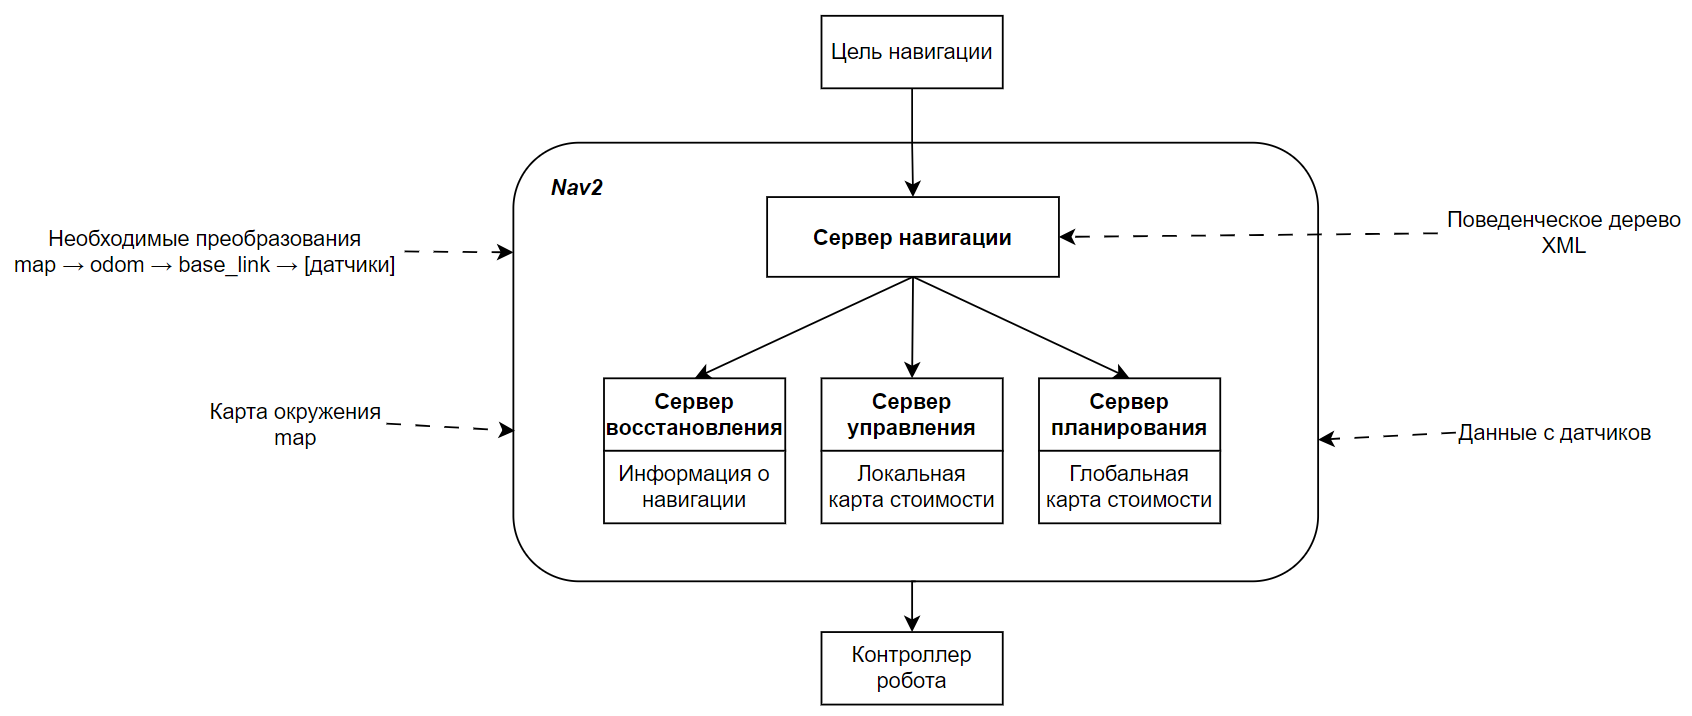
\includegraphics[width=1.0\textwidth]{images/chap_2/nav2_arch.png}
    \caption{Архитектура Nav2}
    \label{fig:nav2_arch}
\end{figure}

Пакеты Nav2 содержат инструменты для сохранения и загрузки карт занятости, локализации робота, планирования траектории, реализации построенной траектории, предоставления локальный и глобальных карт стоимости, реализации некоторого поведения и восстановления робота \cite{ros2-mara}. В эти пакеты часто интегрируется метод одновременной локализации и картографирования (SLAM) из пакета SLAM Toolbox \cite{slam-toolbox}. Возможности планирования и слежения за траекторией, которые соответствуют глобальному и локальному планировщику, дополнительно поддерживаются готовыми плагинами планирования, которые используют алгоритмы A* и Дейкстры для глобального планирования траектории и подходы динамического окна (DWB) или эластичных лент (TEB) для построения и выполнения локального плана. Последовательность работы системы осуществляется по иерархической структуре, реализованной с помощью поведенческого дерева. Основное поведенческое дерево вызывает действия соответствующих планировщиков друг за другом в асинхронном режиме, как показано на Рисунке \ref*{fig:nav2_bt}.

\begin{figure}[h]
    \centering
    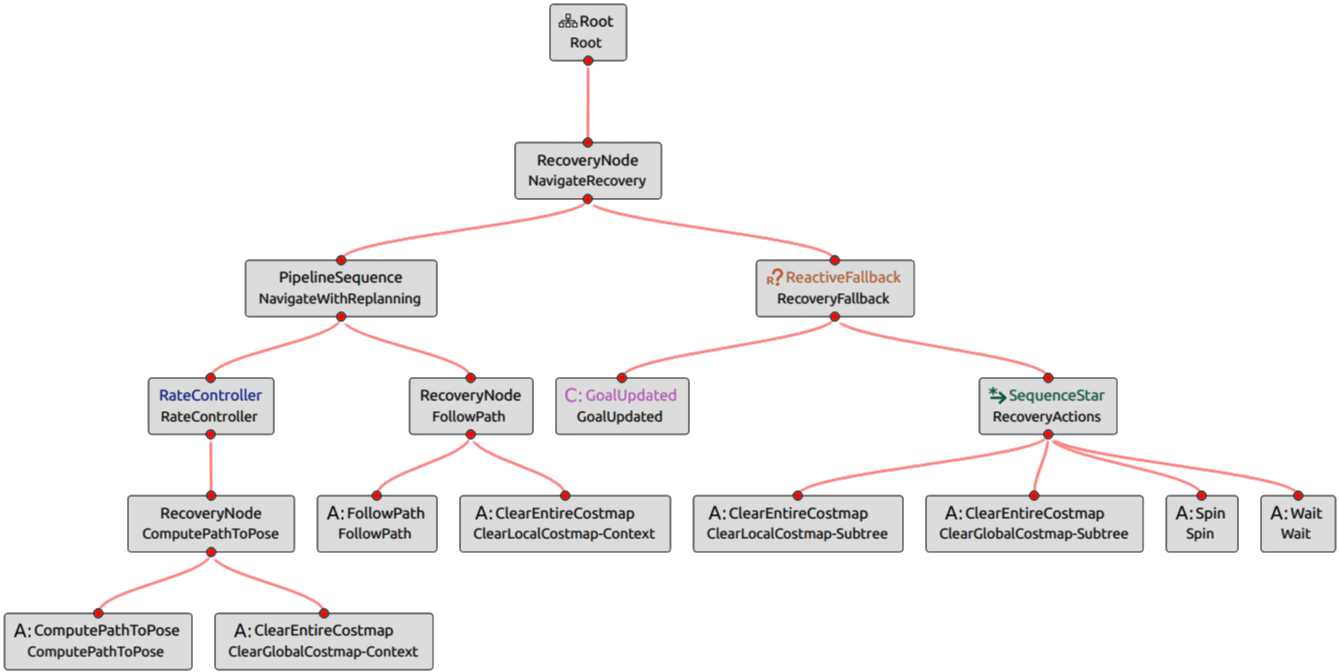
\includegraphics[width=1.0\textwidth]{images/chap_2/nav2_bt.png}
    \caption{Основное поведенческое дерево Nav2}
    \label{fig:nav2_bt}
\end{figure}

Данной поведенческое дерево используется Nav2 по умолчанию и имеет набор уже реализованных поведений восстановления (вращение (spin), ожидание (wait), очистка карты (clear map)). Эти поведения выполняются, если робот не может продвинуться к поставленной цели. 

Также в Nav2 используется система управления жизненным циклом узлов (представленная в ROS2) для контролируемого запуска, активации, деактивации и выключения узлов. Подход, основанный на жизненном цикле, позволяет системе следить за запуском, выполнением и сбоями узлов системы.

\section{Модель робота Turtlebot3}

Turtlebot3 - это стандартная мобильная исследовательская платформа для управления роботом. Робот хорошо интегрирован в экосистему ROS и используется как система для разработки и интеграции новых методов навигации. Робот оснащен двумя двигателями с подключенными к ним энкодерами (дифференциальный привод). Третье колесо стабилизирует робота (т.н. caster wheel).

Производитель ROBOTIS предоставляет модель с открытым исходным кодом для моделирования робота в физических симуляторах, таких как Gazebo, что позволяет ускорить разработку и тестирование создаваемых робототехнических приложений.

Мобильный робот Turtlebot3 обладает всеми необходимыми датчиками для использования Nav2. Технические характеристики робота приведены в Таблице \ref*{tab:tb3_specs}.

\begin{table}[]
    \centering
    \begin{tabular}{|c|c|}
        \hline 
        \textbf{Характеристика} & \textbf{Значение} \\
        \hline
        Максимальная линейная скорость, м/с & 0.26 \\
        \hline
        Максимальная угловая скорость, рад/с & 1.82 \\
        \hline
        Вес, кг & 1.8 \\
        \hline
        Габариты робота, мм & 281x306x141 \\
        \hline
        Одноплатный компьютер & Raspberry Pi 4 \\
        \hline
        Процессов & 32-bit ARM Cortex-M7 \\
        \hline
        Лазерный дальномер & $360^\circ$ LDS-02 \\
        \hline
        RGB-камера & Rapsberry Pi Camera \\
        \hline
        Гироскоп & 3-х осевой\\
        \hline
        Акселерометр & 3-х осевой \\
        \hline
    \end{tabular}
    \caption{Основные технические характеристики Turtlebot3 (waffle-pi)}
    \label{tab:tb3_specs}
\end{table}

\section{Симуляционная среда Gazebo}

Разработка и тестирование системы осуществляется с помощью симулятора Gazebo и модели Turtlebot3. Gazebo хорошо интегрирован в ROS2 и предлагает множество интерфейсов ROS2 для управления симуляцией. 

Симулятор Gazebo точно моделирует физику робота и может публиковать показатели одометрии в соответсвующую тему, также как и показания лазерного сканера и данные с инерциального измерительного блока с помощью соответсвующих плагинов. 

Симулятор обеспечивает более легкую повторяемость тестовых примеров, так как в любой момент можно создать различные препятствия и вызвать сбои датчиков, что приводит к ускорению разработки в целом.

Использование симулятора позволяет замедлить или ускорить время работы со средой. Регулирование времени позволяет более тщательно наблюдать за быстрыми процессами в замедленном режиме, а также наблюдать за устойчивостью системы в течение времени при длительных испытаниях.

\section{Behaviortree.CPP}
ПО Navigation2 использует поведенческое дерево для реализации слоя планирования. Используемое дерево является расширением библиотеки \textit{Behaviortree.CPP}. \\ 
Эта библиотека предлагает способ создания, выполнения, мониторинга и редактирования поведенческих деревьев.

В дополнение к типам управляющих узлов, упомянутых в разделе 1.2.2, библиотека добавляет в каталог управляющих узлов концепцию реактивности. Реактивные узлы последовательности и реактивные селекторы отличаются от обычных тем, что обрабатывают узлы, которые возвращают состояние "Выполняется". Вместо того чтобы ждать пока узел завершит действие, вся последовательность перезапускается, что полезно для непрерывной проверки условия.

Также данная библиотека реализует способ коммуникации между узлами дерева. Для того чтобы узлы дерева могли общаться, библиотека предоставляет разработчику две возможности:
\begin{enumerate}
    \item Любой из узлов может использовать общую доску, реализованную в виде словаря (ключ/значение), которую могут читать и записывать все узлы дерева.
    \item Любые два узла могут быть соединены через порты, что позволяет напрямую связываться между двумя узлами через ключ/значение.
\end{enumerate}

\section{Groot}
Groot - это программа для создания, редактирования, мониторинга и отладки поведенческих деревьев с графическим интерфейсом. Программа позволяет создавать деревья поведения в XML-файлах, которые могут быть напрямую загружены в библиотеку \textit{BehaviorTree.CPP} и использоваться ею. 

Groot может следить за исполнением деревьев поведения в реальном времени и позволяет анализировать реакцию дерева на различные сценарии. На Рисунке \ref*{fig:groot-example} показан небольшой фрагмент поведенческого дерева.

\begin{figure}[h]
    \centering
    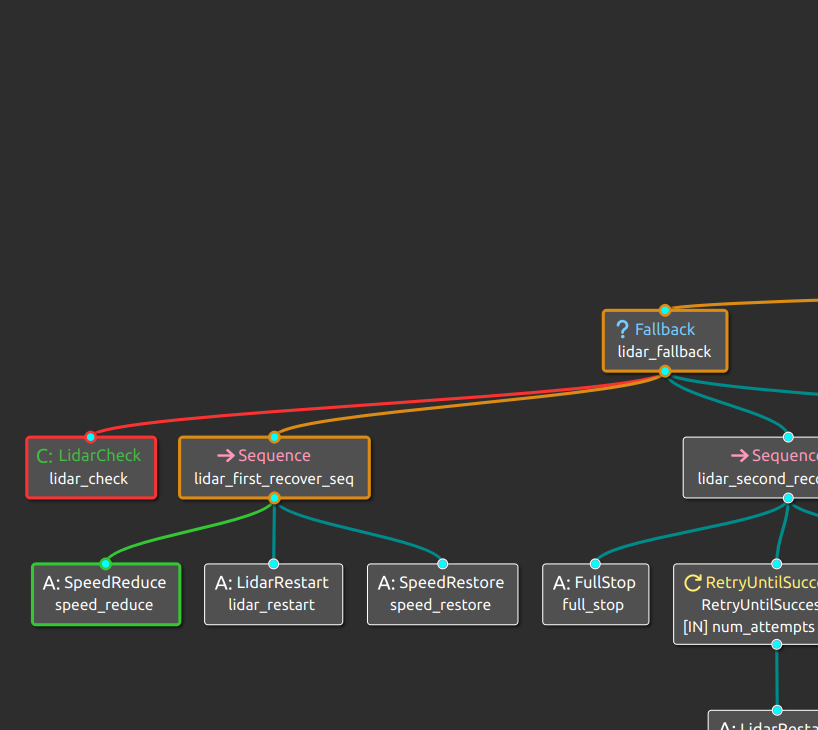
\includegraphics[width=0.7\textwidth]{images/chap_2/groot-example.png}
    \caption{Основное поведенческое дерево Nav2}
    \label{fig:groot-example}
\end{figure}

В этом графическом интерфейсе узлы условий помечены буквой "C" перед названием узла, а узлы действи - буквой "A". Цвета указывают на поток управления и возвращаемые результаты соответствующих узлов. Зеленая рамка вокруг узла показывает, что сигнал управления был обработан и вернул "Успех", а красная рамка сигнализирует о том, что узел вернул "Неудачу". 

В изображенном примере узел "lidar\_check" вернул "Неудачу", далее селектор начал выполнять узел последовательности под названием "lidar\_first\_recover\_seq". Поток управления еще не вернулся обратно в последовательность, поэтому граница последовательности окрашена в оранжевый цвет (состояние "Выполнение"). Изображенное дерево выполняет узел действия в нижней части рисунка с именем "speed\_reduce".

\section{Используемое ПО}

Версии программного обеспечения, использованные для реализации и тестирования системы, перечислены ниже в Таблице \ref*{tab:os_vers}.

\begin{table}[h]
    \centering
    \begin{tabular}{|c|c|}
        \hline
        \textbf{Название} & \textbf{Версия} \\
        \hline
        ОС & Linux, Ubuntu 22.04.4 LTS \\
        \hline
        ROS & ROS2 Humble \\
        \hline
        Nav2 & Nav2, humble-devel (с внесенными изменениями) \\
        \hline
        Симулятор & Gazebo 11 \\
        \hline
        Робот & Turtlebot3 waffle-pi (с внесенными изменениями) \\
        \hline
        BT & BehaviorTree.cpp 3.8 \\
        \hline
        C++ & C++ 14 \\
        \hline
        Python & 3.10.12 \\
        \hline
        Система сборки & CMake, colcon \\
        \hline
        OpenCV & 4.9.0 \\
        \hline
        SciPy & 1.13.0 \\
        \hline
        NumPy & 1.26 \\
        \hline
    \end{tabular}
    \caption{Используемое программное обеспечение}
    \label{tab:os_vers}
\end{table}

\endinput